\documentclass[11pt]{article}
\usepackage[margin=1in]{geometry}
\usepackage{amsmath,amssymb}
\usepackage{graphicx}
\usepackage{booktabs}
\usepackage{array}
\usepackage{float}
\usepackage{hyperref}

\title{Disk Organization and BTFR Scatter\\A Preliminary Test of the Bound Domain Vacuum Response Hypothesis}

\author{Jake Enholm}
\date{}

\begin{document}
\maketitle

\begin{abstract}
The baryonic Tully--Fisher relation (BTFR) links galaxy baryonic mass to rotational velocity with small observed scatter. We test whether part of the observed scatter is associated with unresolved scalar proxies for disk organization and velocity recoverability. The Bound Domain Vacuum Response (BDVR) hypothesis considered here proposes that a dynamical discrepancy may exist in both regular and irregular systems, while greater disk organization produces convergence toward a reproducible BTFR-like relation. We evaluate survey-specific unresolved proxies in selected SPARC and H~I-detected xGASS galaxies. These proxies combine structural variables with inclination, global H~I linewidth, and gas fraction; consequently, they mix possible physical information with observational recoverability and mathematical coupling to the BTFR velocity. The highest- and lowest-ranked proxy quartiles exhibit different observed BTFR residual scatter in both samples, although the intermediate quartiles are not uniformly ordered. In xGASS, the association weakens after controlling for inclination, linewidth, baryonic mass, and measurement quality. The composite proxy adds little predictive information beyond those controls. The present analysis therefore does not provide evidence for a physical BDVR organization coordinate; it shows that the current unresolved proxy is not independent of measurement recoverability. A decisive test requires resolved H~I measurements of rotational dominance, velocity-field symmetry, pressure support, radial convergence, and gas--stellar alignment measured independently of the BTFR velocity.
\end{abstract}

\section{Introduction}

The baryonic Tully--Fisher relation (BTFR) links the total baryonic mass of a disk galaxy to its asymptotic rotation velocity~\cite{mcGaugh2012}. The small observed scatter ($\sim$0.1 dex) indicates a close coupling between baryonic mass and rotational velocity across rotationally supported galaxies. The residual scatter around this relation contains contributions from measurement uncertainty, velocity definition, inclination, baryonic-mass estimates, and genuine diversity in galaxy structure and kinematics~\cite{bradford2016}. Tully and Fisher established the original luminosity--linewidth relation as a galaxy distance indicator~\cite{tully1977}. Later work extended this relation to total baryonic mass, producing the baryonic Tully--Fisher relation used here~\cite{courteau2014, mcGaugh2012}. The BTFR extends into the dwarf-galaxy regime, although pressure support, rising rotation curves, uncertain inclinations, and irregular velocity fields complicate the definition of a characteristic circular velocity~\cite{swaters2009, deblok2010}.

In this paper, we introduce the Bound Domain Vacuum Response (BDVR) response-organization hypothesis as a phenomenological interpretation of the empirical analysis below. The hypothesis proposes that baryonic structure and dynamical organization influence how an additional effective response is expressed through ordered rotation. By dynamical discrepancy we mean the difference between the observed rotation and the Newtonian prediction from the adopted baryonic mass model. The hypothesis does not require this discrepancy to vanish in irregular or weakly settled systems.

The physical idea is simple. BDVR does not require every galaxy with a dynamical discrepancy to lie cleanly on the BTFR. A gas-rich, asymmetric, or pressure-supported system may contain the same underlying response but fail to express it as a single stable rotation velocity. A settled disk, by contrast, should express more of the response as regular, approximately axisymmetric rotation. The observational prediction is therefore not merely that galaxies rotate faster than their visible baryons predict. The prediction is that better-organized disks should show less scatter around the BTFR-like scaling.

The present study evaluates whether unresolved catalog observables can serve as a useful preliminary proxy for later resolved tests. We construct an unresolved organization proxy: a weighted combination of inclination, global H~I linewidth, and atomic gas fraction. We test whether galaxies with higher proxy values show reduced observed scatter around the BTFR. We emphasize at the outset that this proxy is not a direct measurement of disk organization; it combines elements of observational recoverability (high inclination improves projected velocity sensitivity) with possible physical content (low gas fraction and large linewidth correlate with dynamically settled disks). The proxy is not a measurement of the $C_{\rm dyn}$ coordinate defined in Section~2; it is an exploratory candidate proxy intended to guide the design of a later resolved-H~I test.

The plan of the paper is as follows. Section~2 presents the phenomenological BDVR response-organization formulation used to define the observational hypothesis. Section~3 describes competing hypotheses. Section~4 presents the data. Section~5 defines velocity, mass, and proxy definitions. Section~6 describes the statistical methods. Section~7 presents the main results. Section~8 reports confounder and leakage audits. Section~9 discusses cross-survey comparison. Section~10 presents the physical interpretation and alternative explanations. Section~11 presents resolved H~I predictions. Section~12 discusses limitations, and Section~13 concludes.

\section{BDVR Response-Organization Formulation}

We present the BDVR response-organization framework as a phenomenological model. It is not derived from an action or field equation; its purpose is to define a precise hypothesis that can be tested with resolved kinematics.

\subsection{Baryonic acceleration}

The squared baryonic circular speed is obtained by summing the gravitational contributions of the stellar disk, gas disk, and bulge under the adopted axisymmetric mass model:

\begin{equation}
V_{\rm bar}^{2}(r) = V_\star^{2}(r) + V_{\rm gas}^{2}(r) + V_{\rm bulge}^{2}(r),
\label{eq:vbar}
\end{equation}

where $V_\star(r)$ denotes the stellar disk contribution, $V_{\rm bulge}(r)$ is zero for bulgeless systems, and $V_{\rm gas}(r)$ includes the adopted helium correction where appropriate. Each term is a model contribution to the circular speed, not an independently observed velocity. The stellar contribution depends on the adopted stellar mass-to-light ratio. SPARC provides stellar mass profiles computed with a fixed $M/L = 0.5\,M_\odot/L_\odot$ in the 3.6~$\mu$m band; the present analysis uses these profiles directly and does not fit $M/L$ per galaxy. The equivalent radial baryonic acceleration is $a_{\rm bar}(r) = V_{\rm bar}^{2}(r)/r$.

\subsection{Phenomenological BDVR response law}

The total dynamical response beyond the Newtonian baryonic contribution is expressed as:

\begin{equation}
a_{\rm resp}(r) = Q_{\rm eff}(r, \mathbf{g}) \sqrt{a_{\rm bar}(r) \, a_{0}},
\label{eq:aresp}
\end{equation}

where $a_{0}$ is a characteristic acceleration scale, $\mathbf{g}$ denotes galaxy-level structural variables, and $Q_{\rm eff} \geq 0$ is a nonnegative, dimensionless response factor. The present analysis neither derives nor estimates $Q_{\rm eff}$. The square-root acceleration form is shared with established low-acceleration phenomenology~\cite{mcGaugh2004, famaey2012}. The additional BDVR proposition is that the observable expression of the response depends on dynamical organization.

The circular-speed equivalent is:

\begin{equation}
V_{\rm resp}^{2}(r) = Q_{\rm eff}(r,\mathbf{g}) \sqrt{V_{\rm bar}^{2}(r) \, r \, a_{0}}.
\label{eq:vresp}
\end{equation}

The present paper does not test the absolute normalization of this relation; it tests whether organization-dependent BTFR residual variance persists under standard controls.

The total equilibrium circular speed is the sum of baryonic and response contributions:

\begin{equation}
V_{\rm circ}^{2}(r) = V_{\rm bar}^{2}(r) + V_{\rm resp}^{2}(r).
\label{eq:vcirc}
\end{equation}

Equation~\ref{eq:vcirc} is the defining phenomenological decomposition of the model. It is not derived from a relativistic field equation in this paper.

\subsection{Outer BTFR limit}

In the outer regime, where most baryonic mass is enclosed, $V_{\rm bar}^{2}(r) \approx G M_{\rm bar}/r$, and $Q_{\rm eff}$ has approached an outer constant, the response term becomes:

\begin{equation}
V_{\rm resp}^{2} \approx Q_{\rm eff} \sqrt{G M_{\rm bar} \, a_{0}}.
\label{eq:vresp_outer}
\end{equation}

The total circular speed in this limit is:

\begin{equation}
V_{\rm circ}^{2} \approx \frac{G M_{\rm bar}}{r} + Q_{\rm eff} \sqrt{G M_{\rm bar} \, a_{0}}.
\label{eq:vcirc_outer}
\end{equation}

When the response term dominates the declining Newtonian term, the outer velocity approaches:

\begin{equation}
V_{\rm flat}^{2} \approx Q_{\rm eff} \sqrt{G M_{\rm bar} \, a_{0}},
\label{eq:vflat_intermediate}
\end{equation}

and hence the flat-velocity baryonic scaling:

\begin{equation}
V_{\rm flat}^{4} \approx Q_{\rm eff}^{2} G M_{\rm bar} \, a_{0}.
\label{eq:vflat_bdvr}
\end{equation}

This derivation assumes: (i) most baryonic mass is enclosed at the radius where $V_{\rm flat}$ is measured; (ii) $Q_{\rm eff}$ has converged to a radially constant value; (iii) the response term is large compared with the declining Newtonian term; (iv) pressure and non-circular corrections are small. Under these conditions the response asymptotically yields a BTFR-like baryonic-mass scaling.

At fixed baryonic mass and fixed $a_{0}$, variations in $Q_{\rm eff}$ contribute additional BTFR scatter:

\begin{equation}
\Delta\log V_{\rm flat} = \frac{1}{2}\Delta\log Q_{\rm eff}.
\label{eq:qeff_scatter}
\end{equation}

\subsection{Equilibrium circular speed and observed rotation}

The observed ordered rotation velocity $V_{\rm rot}$ is not necessarily identical to the equilibrium circular speed $V_{\rm circ}$. We distinguish two models.

First, the equilibrium model is simply Eq.~\ref{eq:vcirc}.

Second, the observational recovery model relates the observed velocity to the equilibrium speed:

\begin{equation}
V_{\rm rot,obs}^{2}(r) \approx V_{\rm circ}^{2}(r) - \Delta_{\rm AD}(r) + \delta_{\rm sys}(r),
\label{eq:obs_recovery}
\end{equation}

where $\Delta_{\rm AD}(r) \geq 0$ is the pressure-support correction required to recover the circular speed from the measured rotation, and $\delta_{\rm sys}(r)$ is a signed residual representing non-circular motions, projection errors, beam smearing, or model inadequacy. Rearranging:

\begin{equation}
V_{\rm circ}^{2}(r) \approx V_{\rm rot,obs}^{2}(r) + \Delta_{\rm AD}(r) - \delta_{\rm sys}(r).
\label{eq:circ_from_obs}
\end{equation}

For a thin gas disk, an illustrative asymmetric-drift-like correction is

\begin{equation}
\Delta_{\rm AD} \approx -\sigma_R^2 \, \frac{\partial\ln(\Sigma_g \sigma_R^2)}{\partial\ln r},
\end{equation}

under assumptions of axisymmetry and a simplified anisotropy model. This correction is not applied in the present scalar-proxy analysis.

We define a BDVR organization coordinate $0 \leq C_{\rm BDVR} \leq 1$. $C_{\rm BDVR}$ does not directly rescale gravity in the present observational model. It is a latent theoretical coordinate describing the degree to which the BDVR response is expressed through regular disk rotation. It is not measured in the present study. As $C_{\rm BDVR} \rightarrow 1$, the fractional contributions of pressure support, non-circular motion, and model-recovery error are hypothesized to become smaller, and the observed ordered rotation more closely approximates the equilibrium circular speed.

\subsection{BDVR Response-Organization Hypothesis}

The BDVR response-organization hypothesis is that the discrepancy between observed dynamics and the Newtonian prediction of the adopted baryonic mass model may occur in both regular and irregular galaxies. The BDVR hypothesis proposes that dynamical organization influences the degree to which this response is represented by regular, approximately axisymmetric rotation. As organization increases, a scalar rotation velocity should more closely approximate the equilibrium circular speed and should exhibit less scatter around the BTFR-like scaling derived above.

\subsection{Scatter prediction}

The central statistical prediction is that BTFR residual variance decreases with increasing response organization:

\begin{equation}
\operatorname{Var}\left[ \Delta_{\rm BTFR} \mid C_{\rm BDVR} \right] \downarrow \quad \text{as} \quad C_{\rm BDVR} \uparrow.
\label{eq:pred_var}
\end{equation}

One possible continuous parameterization is an exponentially declining conditional-variance model:

\begin{equation}
\sigma_{\Delta}^{2}(C_{\rm BDVR}) = \sigma_{\rm floor}^{2} + \sigma_{\rm unsettled}^{2} \exp(-\gamma \, C_{\rm BDVR}), \quad \gamma > 0,
\label{eq:var_model}
\end{equation}

where $\sigma_{\rm floor}$ is the asymptotic minimum scatter as organization becomes large in the chosen parameterization, and $\sigma_{\rm unsettled}$ is the additional scatter at $C_{\rm BDVR}=0$, so that $\sigma_{\Delta}^2(0) = \sigma_{\rm floor}^2 + \sigma_{\rm unsettled}^2$ and $\sigma_{\Delta}^2(1) = \sigma_{\rm floor}^2 + \sigma_{\rm unsettled}^2 e^{-\gamma}$. This equation is proposed for future resolved analysis and is not fitted in the present scalar-proxy study. In a future resolved analysis that fits this parameterization, the BDVR response-organization prediction would be $\gamma > 0$ after controlling for mass, inclination, velocity uncertainty, distance uncertainty, profile quality, and survey selection.

The BDVR framework is used here only to motivate a falsifiable organization hypothesis. The empirical tests below do not measure $Q_{\rm eff}$, do not infer a galaxy-by-galaxy BDVR coupling strength, and do not distinguish a new response law from conventional disk-settling physics. They test whether unresolved scalar observables can identify galaxies with reduced BTFR residual scatter and whether those observables are worth using for target selection in a resolved-H~I follow-up program.

\section{Competing Hypotheses}

The response-organization hypothesis is distinct from several alternatives that must be tested simultaneously:

\begin{enumerate}
\item \textbf{Measurement-recoverability hypothesis}: the apparent scatter reduction reflects the fact that the BTFR velocity is measured more reliably for edge-on, high-linewidth galaxies, not that these galaxies are physically more converged.
\item \textbf{Mass-dependent scatter hypothesis}: the observed BTFR residual variance may increase toward low masses because of both measurement uncertainty and physical diversity, and the candidate proxy correlates with mass.
\item \textbf{Gas-richness hypothesis}: gas-dominated galaxies have larger scatter because their baryonic mass is harder to measure or their dynamics are genuinely more diverse.
\item \textbf{Conventional disk settling}: established galaxy-formation physics predicts that low-mass, gas-rich galaxies have more diverse dynamics through standard angular-momentum acquisition, turbulent-to-rotational support transition, and feedback processes, without invoking a new dynamical response. Modern hydrodynamic simulations and high-redshift kinematic surveys demonstrate that disks emerge from turbulent gas through a gradual settling process that spans a range of dynamical states~\cite{pillepich2019, wisnioski2015}.
\end{enumerate}

The present analysis tests whether the observed scatter--proxy association survives controls for these alternatives. The scalar proxy is presented as a candidate selection diagnostic for later resolved-H~I tests, not as a direct measurement of the $C_{\rm BDVR}$ coordinate defined above.

\section{Data}

\subsection{SPARC}

SPARC~\cite{lelli2016} contains 175 galaxies with published rotation curves, stellar and gas mass profiles, and surface photometry. Table~\ref{tab:sparc_selection} summarizes the sample selection:

\begin{table}[H]
\centering
\caption{SPARC sample selection for the present scalar-proxy analysis. Selection counts refer to the variables and parsed inputs available in the current local analysis table.}
\label{tab:sparc_selection}
\begin{tabular}{lrr}
\toprule
Selection step & Excluded & Remaining \\
\midrule
SPARC parent catalog & 0 & 175 \\
Missing $V_{\rm flat}$ & 88 & 87 \\
Missing baryonic mass variables & 0 & 87 \\
Missing proxy inputs ($\Sigma, f_*, R_{\rm HI}/R_d$) & 0 & 87 \\
\bottomrule
\end{tabular}
\end{table}

We select 87 for the present analysis after requiring: available baryonic mass variables, a measured rotation velocity, and complete proxy inputs. We use scalar measurements including the gas fraction $f_{\rm gas}$, the stellar fraction $f_*$, the stellar surface density $\log_{10}\Sigma$, and the BTFR offset $\Delta_{\rm BTFR}$ from the earlier analysis adopting the McGaugh (2012) calibration. Our local Rotmod decomposition pipeline currently contains 25 successfully parsed rotation-curve models; the remaining 62 galaxies enter only through their scalar summary quantities. We treat this as a limitation of the present analysis, not as a statement about the full SPARC archive.

\subsection{xGASS}

xGASS~\cite{catinella2018} is a stellar-mass-selected survey of approximately 1,200 nearby galaxies with H~I detections and nondetections. xGASS extends the original GASS atomic-gas survey to lower stellar masses; COLD GASS provides molecular-gas measurements for an overlapping sample~\cite{saintonge2011}. Quality cuts (HI\_FLAG=1, INCL $>30^\circ$) select 363 galaxies with clean global H~I profiles. Cross-validated results using training-set data are reported separately.

\section{Velocity and Baryonic-Mass Definitions}

\subsection{Velocity conventions}

The BTFR requires a characteristic rotation velocity. We distinguish:

\begin{itemize}
\item $W_{50}$: the global H~I linewidth at 50\% of peak flux, uncorrected for inclination. This is the primary velocity proxy for the xGASS analysis.
\item $V_{\rm rot} = W_{50} / (2\\sin i)$: the inclination-corrected linewidth, used as the BTFR velocity after a small turbulence correction (Eq.~\ref{eq:width_corr}).
\item $V_{\rm flat}$: the asymptotic flat rotation velocity from resolved rotation curves (SPARC).
\end{itemize}

These quantities are not interchangeable. The BTFR is calibrated on $V_{\rm flat}$, but the global $W_{50}$ depends on inclination, turbulent broadening, and profile shape in ways that $V_{\rm flat}$ does not (see~\cite{ponomareva2018} for a detailed comparison of velocity definitions; see also~\cite{lelli2019} for a systematic comparison of BTFR behavior under different velocity definitions in SPARC).

\subsection{Velocity corrections}

We treat the correction procedure as a limitation, because the adopted turbulence correction is a uniform estimate rather than a per-galaxy measurement.

The inclination-corrected linewidth is computed as:

\begin{equation}
W_{\rm corr} = \sqrt{W_{50}^2 - W_{\rm turb}^2},\label{eq:width_corr}
\end{equation}

with the adopted turbulence correction $W_{\rm turb} = 10\,{\rm km\,s}^{-1}$ following~\cite{bradford2016}. This correction is applied only when $W_{50} > W_{\rm turb}$; no analyzed object falls below this threshold. We adopt this simplified quadratic correction for the present exploratory analysis. For linewidths in this regime, it broadly approximates more detailed methods~\cite{springob2005}.

\begin{equation}
V_{\rm rot} = \frac{W_{\rm corr}}{2\sin i},\label{eq:vrot}
\end{equation}

where $i$ is the inclination. We did not apply additional instrumental-resolution or rest-frame width corrections.

\subsection{BTFR convention}

We fit the BTFR with rotation velocity as a function of baryonic mass (velocity-on-mass):

\begin{equation}
\log_{10} V = a \log_{10} M_{\rm bar} + b,
\end{equation}

where $M_{\rm bar} = M_* + 1.33 M_{\rm HI}$ (our adopted stars-plus-atomic-gas mass). This sum includes atomic gas with a helium correction factor of 1.33 and omits molecular gas and ionized gas, which are not uniformly available for the full sample.

We fit velocity as a function of baryonic mass because the present analysis defines residuals in the velocity coordinate. The slope $a=0.299$ corresponds to an inverse-form mass slope $\alpha \approx 1/a \approx 3.34$, within the range commonly reported for baryonic Tully--Fisher fits, although the fitted slope depends on velocity definition, sample selection, regression direction, and treatment of measurement error. The reciprocal of a fitted velocity-on-mass slope is not generally identical to a separately fitted mass-on-velocity slope in the presence of scatter and measurement error. Reported scatter is the standard deviation of signed residuals around the fitted relation.

The BTFR is fitted inside cross-validation folds for the primary xGASS analysis (Section~6) and globally for comparison with published relations. Residuals are computed as $\Delta_{\rm BTFR} = \log_{10} V_{\rm obs} - \log_{10} V_{\rm pred}$.

For SPARC, we use the BTFR calibration \cite{mcGaugh2012}.
For xGASS, held-out residual scatter is the primary dispersion metric; no correction for measurement uncertainty is applied.

\section{Scalar Organization Proxy}

\subsection{xGASS proxy}

The primary organization proxy for xGASS combines three terms:

\begin{equation}
\mathcal{C}_{\rm xGASS} =
0.35 \left(\frac{i}{90^\circ}\right)
+ 0.35 \left(\frac{W_{50} - W_{50,\min}}{W_{50,\max} - W_{50,\min}}
\right)
+ 0.30 (1 - f_{\rm atm}),
\end{equation}

where $i$ is the inclination, $W_{50}$ the global H~I linewidth, and $f_{\rm atm}$ the atomic gas fraction $M_{\rm HI}/M_{\rm bar}$. The inclination term $i/90^\circ$ is an edge-on ranking (observational recoverability), not a physical organization measurement. The min--max normalization of $W_{50}$ was computed using the full dataset; this leaks held-out information into the score and must be estimated inside training folds in a fully fold-local analysis. The weights (0.35, 0.35, 0.30) are heuristic and were not optimized. The resulting score should be understood as a heuristic index, not a fitted model. We note that the raw $W_{50}$ component couples the proxy to the same linewidth used in the BTFR velocity (Eq.~\ref{eq:vrot}), so this component does not constitute independent evidence of physical organization. Section~9 tests the sensitivity of the result to alternative formulations.

\subsection{SPARC proxy}

For SPARC, where resolved information is available but uneven across the sample, we construct a composite demographic organization index from standardized predictors:

\begin{equation}
z_j = \frac{x_j - \operatorname{median}(x_j)}{\operatorname{MAD}(x_j)},
\end{equation}

\begin{equation}
\mathcal{D}_{\rm SPARC} = w_1 z_{\log\Sigma} + w_2 z_{f_*} - w_3 z_{R_{\rm HI}/R_d},
\end{equation}

where $\Sigma$ is the stellar surface density, $f_*$ the stellar fraction, $R_{\rm HI}/R_d$ the H~I-to-optical disk scale-length ratio (larger values indicate more extended gas disks, which we assume correspond to lower dynamical organization), MAD denotes the median absolute deviation (a robust dispersion estimator), and $w_j = 1/3$ are equal weights. The stellar surface density is the central value as reported in the SPARC catalog; $R_{\rm HI}$ is defined at the $1\,M_\odot\,{\rm pc}^{-2}$ column-density threshold following standard H~I disk conventions. The resulting score is normalized to $[0,1]$ via min--max scaling. Because $f_* + f_{\rm gas} \approx 1$, the gas fraction is implicitly included through the stellar fraction. The stellar surface density is taken from the SPARC $\log$SB column. We emphasize that this is a demographic organization index, not a direct disk organization measurement.

\subsection{Three distinct coherence quantities}

We distinguish three related but distinct quantities:

\begin{enumerate}

\item \textbf{$C_{\rm proxy}$} (empirical unresolved proxy). This is the numerical score constructed from linewidth, inclination, and gas fraction ($\mathcal{C}_{\rm xGASS}$, $\mathcal{D}_{\rm SPARC}$). It is an observational recoverability diagnostic, not a physical organization measurement. It does not require the BDVR framework to interpret.

\item \textbf{$C_{\rm dyn}$} (direct dynamical organization). This is a future resolved-H~I quantity constructed from physical kinematic measurements of velocity-field symmetry, rotational dominance, pressure support, and convergence.

\item \textbf{$C_{\rm BDVR}$} (latent theoretical coordinate). This is the $0 \leq C_{\rm BDVR} \leq 1$ coordinate defined in Section~2 that describes the degree to which the BDVR response is expressed through regular disk rotation. It is not measured in the present study. The scalar proxies serve as a preliminary recoverability test of candidate proxy utility, not as a direct $C_{\rm BDVR}$ measurement.

\end{enumerate}

These three quantities are not equivalent:

\begin{equation}
C_{\rm proxy} \not\equiv C_{\rm dyn} \not\equiv C_{\rm BDVR}.
\label{eq:neq_coherence}
\end{equation}

The analysis below uses $C_{\rm proxy}$. References to ``the proxy'' refer to this empirical unresolved score unless otherwise specified. Galaxies are divided into quartiles: Q1 (lowest proxy value) through Q4 (highest proxy value).


\section{Statistical Methods and Validation Design}

\subsection{Analysis target}

The central question is whether the scatter in BTFR residuals decreases with increasing organization. The primary object-level target is the absolute residual $|\Delta_{\rm BTFR}|$. Quartile scatter ratios $\sigma_{Q4}/\sigma_{Q1}$ provide a descriptive summary, and Spearman rank correlations between $C_{\rm proxy}$ and $|\Delta_{\rm BTFR}|$ quantify the monotonic association. Throughout this paper, negative Spearman $\rho$ is the expected direction: higher proxy value corresponds to lower absolute BTFR residual.

\subsection{Cross-validation}

To reduce target leakage in the BTFR residual calculation, the BTFR is fitted inside 5-fold cross-validation for xGASS. In each fold, the relation is calibrated on the training set only, held-out absolute residuals are recorded, and the organization--scatter association is evaluated on held-out galaxies. In the current implementation, the proxy normalization uses full-sample extrema rather than fold-local estimates. A fully leakage-free implementation would estimate all transformations within each training fold. Therefore these results should be described as cross-validated BTFR residual results, not as a fully leakage-free predictive validation.

\subsection{Bootstrap confidence intervals}

Confidence intervals for scatter ratios are computed by bootstrap (1,000 replications with replacement).

\subsection{Confounder audits}

We perform the following audits (Section~9): organization-proxy ablation (full proxy + six variants), inclination-restricted analysis ($i=45^\circ$--$75^\circ$ and $50^\circ$--$80^\circ$), mass-residualized and mass-matched comparisons, and measurement-quality regression controls.

\subsection{Null models}

We compare the full organization proxy against six alternative models: inclination only, $W_{50}$ only, gas fraction only, baryonic mass, stellar mass, and a combined model of mass, inclination, and quality flags.

\section{Results}

\subsection{SPARC}

In SPARC, galaxies in the highest organization quartile (Q4) show 35\% lower $|\Delta_{\rm BTFR}|$ scatter than the lowest quartile (Q1): $\sigma_{Q1} = 0.0753$ dex, $\sigma_{Q4} = 0.049$ dex, Q4/Q1 = 0.65 (Figure~\ref{fig:scatter_quartile}). The intermediate quartiles are not uniformly monotonic, and the modest sample size ($N=87$) limits statistical precision. Because the SPARC and xGASS proxies are different constructions and neither directly measures resolved disk organization, the endpoint scatter reduction should be interpreted as a preliminary proxy result rather than as a physical organization measurement.

\subsection{xGASS: full-sample result}

With the kinematics-driven coherence model, xGASS shows a larger scatter reduction: Q4/Q1 = 0.38 (Spearman $\rho = -0.238$), with the highest-ranked quartile having 62\% lower scatter than the lowest. Of the 363 xGASS galaxies, 320 have all quantities required for the inclination-corrected $V_{\rm rot}$ analysis; the remaining 43 lack derived $V_{\rm rot}$ in the current analysis table and are shown separately as a W50-only diagnostic subset (Figure~\ref{fig:scatter_quartile}, right panel). This subset is not treated as a full-sample replication of the main xGASS result.

\subsection{Cross-validated result}

When the BTFR is fitted inside 5-fold cross-validation, the held-out scatter ratio is Q4/Q1 = 0.365 (95\% CI: [0.231, 0.572], Spearman $\rho = -0.285$). The effect survives cross-validated BTFR fitting, with a held-out scatter ratio comparable to the full-sample estimate.

\section{Confounder and Leakage Audits}

\subsection{Proxy ablation}

We evaluated the full proxy and six ablation variants to identify the source of the scatter--organization association (Table~2). Key results:

\begin{itemize}
\item Inclination alone produces a Spearman $\rho = -0.352$, indicating that the edge-on ranking accounts for a substantial fraction of the observed correlation.
\item Removing raw $W_{50}$ from the proxy reduces the correlation by approximately 40\% ($\rho = -0.142$).
\item Linewidth alone yields $\rho = -0.237$, which raises the concern that the $W_{50}$ used in the proxy is mathematically related to the velocity used in the BTFR.
\item Gas fraction alone has the \emph{opposite} sign (higher gas fraction associated with higher scatter), indicating that the gas term in the full proxy is not the driver of the effect.
\item The variant combining inclination and $W_{50}$ only (removing gas fraction) produces the strongest correlation, confirming that the association is primarily driven by orientation and linewidth terms.
\end{itemize}

The strongest variant (Inclination + W50) is also the least physically independent, because it is built entirely from inclination and linewidth.

These results imply that the observed scatter reduction is strongest for proxies containing inclination and linewidth information and weaker or absent for demographic proxies. This is consistent with both a measurement-quality interpretation (high inclination and broad profiles improve the recoverability of projected rotation) and a physical interpretation (these same properties may correlate with mass or disk structure).

Table~\ref{tab:ablation} summarizes the full ablation results.

\begin{table}[H]
\centering
\caption{Organization proxy ablation results in xGASS. Variants are listed with their Spearman correlation against $|\Delta_{\rm BTFR}|$, Q4/Q1 scatter ratio, and 95\% bootstrap confidence interval. Kinematics variants include inclination and/or linewidth; these carry the highest leakage risk because the same velocity proxies enter the BTFR.}
\label{tab:ablation}
\begin{tabular}{lccrr}
\toprule
Proxy variant & Features & $\rho$ & Q4/Q1 & 95\% CI \\\midrule
Inclination + linewidth + gas fraction & i+W50+gas & -0.213 & 0.411 & [0.256, 0.63] \\No W50 & i+gas & -0.142 & 0.628 & [0.284, 1.04] \\No inclination & W50+gas & -0.047 & 0.46 & [0.312, 0.761] \\Inclination only & i & -0.352 & 0.459 & [0.213, 0.807] \\W50 only & W50 & -0.237 & 0.481 & [0.305, 0.661] \\Inclination + W50 & i+W50 & -0.353 & 0.29 & [0.2, 0.46] \\Gas only & $f_{\rm atm}$ & 0.225 & 1.54 & [0.923, 3.08] \\\bottomrule
\end{tabular}

\smallskip
\noindent{}\textit{Note.} Negative Spearman $\rho$ indicates that higher proxy value is associated with lower absolute BTFR residual. Q4/Q1 $<$ 1 indicates lower scatter in the highest organization-proxy quartile than in the lowest quartile.
\end{table}

\subsection{Inclination-restricted analysis}

To separate the edge-on ranking from possible physical organization, we repeated the analysis in restricted inclination ranges:

\begin{itemize}
\item Full range ($0^\circ < i < 90^\circ$): Spearman $\rho(i, |\Delta_{\rm BTFR}|) = -0.352$.
\item Mid range ($45^\circ < i < 75^\circ$, N=231): Q4/Q1 = 0.561 (CI: [0.331, 0.887]).
\item Mid range ($50^\circ < i < 80^\circ$, N=224): Q4/Q1 = 0.525 (CI: [0.333, 0.871]).
\end{itemize}

The scatter reduction persists in the restricted inclination range but is substantially weaker, showing that orientation contributes materially to the observed effect. The 95\% confidence intervals do not include unity.

\subsection{Mass controls}

Baryonic mass correlates with both the scalar proxy and BTFR scatter. After residualizing the proxy against $\log M_{\rm bar}$, the Spearman correlation drops from $\rho = -0.213$ to $\rho = -0.14$. Mass-matched quartiles (within narrow $\log M_{\rm bar}$ bins) give a scatter ratio of 0.46. In a linear model predicting $|\Delta_{\rm BTFR}|$ from $C_{\rm proxy}$, $\log M_{\rm bar}$, and their interaction, the interaction coefficient is 0.117 $\pm$ 0.085 ($t \approx 1.4$, $p \approx 0.17$). The mass--organization interaction is therefore consistent with zero, suggesting that the organization--scatter relationship does not strongly vary with mass. The matching uses baryonic mass with fixed-width bins and nearest-neighbor assignment without replacement. The association is therefore not fully explained by the tested mass correlation alone, but mass is a significant confounder.

\subsection{Measurement-quality controls}

We fitted linear models predicting $|\Delta_{\rm BTFR}|$ from basic quality-related variables (baryonic mass, inclination, axis ratio $b/a$, and H~I confusion flag). The null model achieves $R^2 = 0.147$. Adding the full organization proxy increases $R^2$ to 0.151 ($\Delta R^2 = 0.0035$). The improvement is marginal. Once basic quality controls are included, the proxy adds almost no predictive power.

\subsection{Summary of confounder audits}

The audits identify three findings that must be reconciled with any physical interpretation:

\begin{enumerate}
\item The edge-on ranking drives a large fraction of the observed scatter reduction.
\item The organization proxy is dominated by the same inclination and linewidth information that enters measurement reliability and mathematical coupling.
\item Quality-controlled regression models show negligible improvement when the organization proxy is added, implying that the proxy does not capture physically independent information beyond what standard observables already provide.
\end{enumerate}

These results do not refute the response-organization hypothesis, but they establish that the current scalar proxy cannot distinguish it from the measurement-quality alternative.

\section{Cross-Survey Comparison}

\subsection{Cross-survey directional consistency}

SPARC and xGASS probe different BTFR regimes with different velocity definitions, mass conventions, and organization proxies. Direct comparison of absolute scatter values (dex) between surveys is not meaningful. Instead, we compare the normalized scatter ratio $\sigma_{Q4}/\sigma_{Q1}$ within each survey.

Both surveys show directional cross-survey consistency: the highest-organization quartile has lower scatter than the lowest in both SPARC and xGASS. The effect is more pronounced in xGASS (62\% reduction) than in SPARC (35\% reduction), but the surveys use different proxies and sample different mass ranges, so this is not an independent replication of the same metric. The directional consistency of the endpoint contrast is notable, but the quantitative difference underscores the proxy-specific nature of the result.

\section{Interpretation and Alternative Explanations}

The subsections below progress from directly observed to increasingly speculative:

\subsection{Directly Observed}

BTFR residual scatter differs across quartiles of the organization proxy in both SPARC and xGASS. The direction is consistent: higher proxy values correspond to lower scatter.

\subsection{Observational Interpretation}

The scalar proxy identifies galaxies whose global H~I velocity is more reliably measured or more rotation-dominated. Edge-on, high-linewidth galaxies produce cleaner projected velocity signals, reducing measurement-driven scatter in the BTFR.

\subsection{Physical Interpretation}

More dynamically settled disks (those with more regular, rotation-supported kinematics rather than irregular, pressure-supported dynamics) may converge toward a reproducible BTFR channel.

\subsection{BDVR Interpretation}

The BDVR hypothesis proposes that baryonic organization may influence the form in which the dynamical response is expressed, so that more settled systems show a cleaner scalar rotation signal than irregular or pressure-supported systems. The scalar proxy is hypothesized to describe the degree of this organization.

The latter two interpretations are not demonstrated by the current data. Three alternative explanations remain viable:

\begin{itemize}
\item \textbf{Measurement systematics:} the BTFR scatter is inflated by measurement error at low inclination or low linewidth; the proxy identifies galaxies with the smallest measurement errors.
\item \textbf{Conventional disk settling:} established galaxy-formation physics predicts that low-mass, gas-rich galaxies have more diverse dynamics~\cite{navarro1997, mo1998}; the proxy assigns lower values to many of these objects.
\item \textbf{Mathematical coupling:} the same linewidth appears in both the proxy and the BTFR velocity, creating a statistical artifact.
\end{itemize}

\section{Resolved H~I Predictions}
\label{sec:resolved_predictions}

The decisive test requires direct measurements of velocity-field coherence from resolved H~I interferometry~\cite{verheijen2001, bosma1978}. Surveys such as THINGS~\cite{walter2008} and LITTLE THINGS~\cite{oh2015} provide the resolved kinematics needed for this test. We outline the following testable predictions:

\paragraph{Prediction 1 (proxy validation).} Scalar high-organization galaxies should show more regular resolved H~I velocity fields than scalar low-organization galaxies matched in baryonic mass, inclination, and measurement quality.

\paragraph{Prediction 2 (organization outliers).} Galaxies assigned high organization by the scalar proxy but showing large BTFR residuals must, if the proxy is physically meaningful, display axisymmetric rotation curves with a systematically offset amplitude (e.g., anomalous $V_{\rm flat}/W_{50}$ ratios). If instead their kinematics are disturbed, the scalar proxy is not a valid tracer of underlying disk organization.

\paragraph{Prediction 3 (resolved curves strengthen the pattern).} The magnitude of the Spearman correlation between resolved organization and BTFR scatter should increase when global linewidths are replaced by resolved rotation curves for the same galaxies. Quantitatively: $|\rho_{\rm resolved}| > |\rho_{W50}|$ and/or $(\sigma_{Q4}/\sigma_{Q1})_{\rm resolved} < (\sigma_{Q4}/\sigma_{Q1})_{W50}$.

\paragraph{Prediction 4 (dwarf-galaxy scatter).} Low-mass, gas-rich samples should show a broader distribution of response organization. Resolved high-organization dwarfs, if present, should occupy a tighter BTFR channel than low-organization dwarfs.

\paragraph{Failure criteria.} The response-organization hypothesis fails if: (1) the scatter effect disappears after inclination and linewidth-quality matching; (2) the scalar score does not predict resolved H~I organization; (3) resolved organization adds no held-out information beyond ordinary quality flags; (4) low- and high-organization galaxies have indistinguishable BTFR residual variance after measurement-error correction; (5) the result depends on using the same velocity quantity in both predictor and target; (6) leave-one-survey-out validation fails.

\section{Limitations}

This analysis has several important limitations:

\begin{enumerate}
\item The organization proxy is not a direct measurement of disk organization. It combines inclination, global linewidth, and gas fraction in a weighted sum whose weights were not optimized or cross-validated.
\item The SPARC and xGASS proxies are different constructions, preventing direct cross-survey replication with the same metric.
\item Measurement-error models for the BTFR are not included; the observed scatter includes both physical and measurement contributions.
\item The sample is limited to relatively massive galaxies ($M_* > 10^9\,M_\odot$ for xGASS). Extension to the dwarf regime requires resolved H~I data.
\item Molecular gas (CO) is not included in the baryonic mass budget for xGASS; the BTFR scatter may be inflated by the absence of this component.
\item The proxy preprocessing (standardization, min--max scaling, and quartile binning) uses the full sample rather than fold-local estimates, which may introduce optimistic bias in the cross-validation results.
\end{enumerate}

\section{Conclusions}

We formulate the BDVR response-organization hypothesis as a distinction between the existence of dynamical excess and the degree to which that excess is represented by regular, rotation-dominated disk motion. In the outer response-dominated limit, the phenomenological BDVR acceleration law approaches a BTFR-like mass--velocity scaling. The present observational analysis does not measure the proposed BDVR organization coordinate directly. Instead, it evaluates unresolved survey-specific proxies that mix gas fraction and linewidth information with inclination-dependent recoverability.

The present analysis finds a repeatable endpoint contrast: galaxies ranked high by unresolved organization proxies show lower observed BTFR residual scatter than galaxies ranked low. However, the strongest proxy components are inclination and linewidth. These quantities are tied to velocity recoverability and, in the case of linewidth, mathematically coupled to the BTFR velocity itself. After basic quality controls, the composite proxy adds negligible explanatory power ($\Delta R^2 \approx 0.0035$). The scalar proxy therefore should not be interpreted as evidence for a physical BDVR organization coordinate. Its value is narrower: it identifies a candidate-selection strategy for a resolved-H~I test in which disk organization can be measured independently of the BTFR velocity.

The decisive test is a resolved analysis in which velocity-field symmetry, rotational dominance, pressure support, radial convergence, and gas--stellar alignment are measured independently of the BTFR velocity. The BDVR response-organization hypothesis predicts that these direct quantities should explain a decrease in BTFR residual variance after mass and measurement uncertainty are controlled.

\section*{Data and Code Availability}

The analysis scripts, input tables, and generated figures are available at the project repository (repository URL to be added after packaging and archival review). The SPARC data are public~\cite{lelli2016}. The xGASS catalog is available at \url{https://xgass.icrar.org}.

\begin{figure}[H]
\centering
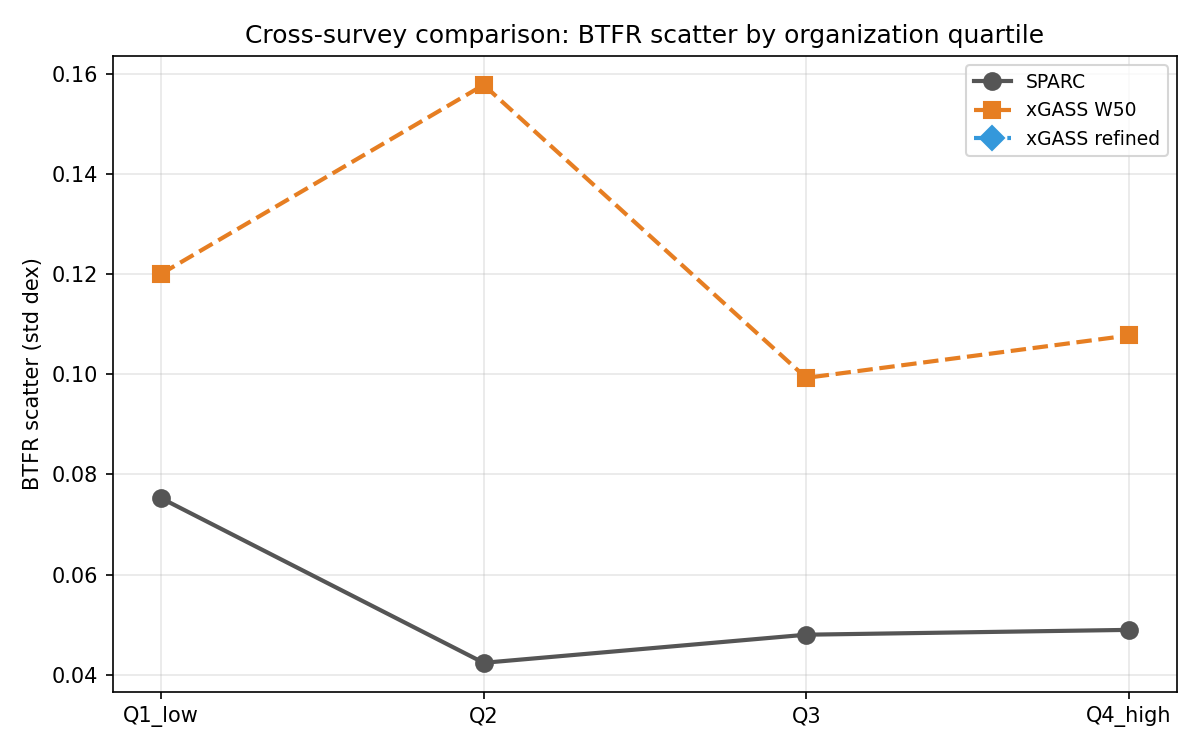
\includegraphics[width=0.85\textwidth]{figures/fig_1_sample_flow.png}
\caption{Cross-survey comparison of BTFR residual scatter by organization quartile. Lines show SPARC and xGASS variants. Because the surveys use different velocity definitions, mass conventions, and proxy constructions, the absolute scatter values should not be compared directly across surveys; the within-survey Q4/Q1 contrast is the relevant quantity.}
\label{fig:cross_comparison}
\end{figure}

\begin{figure}[H]
\centering
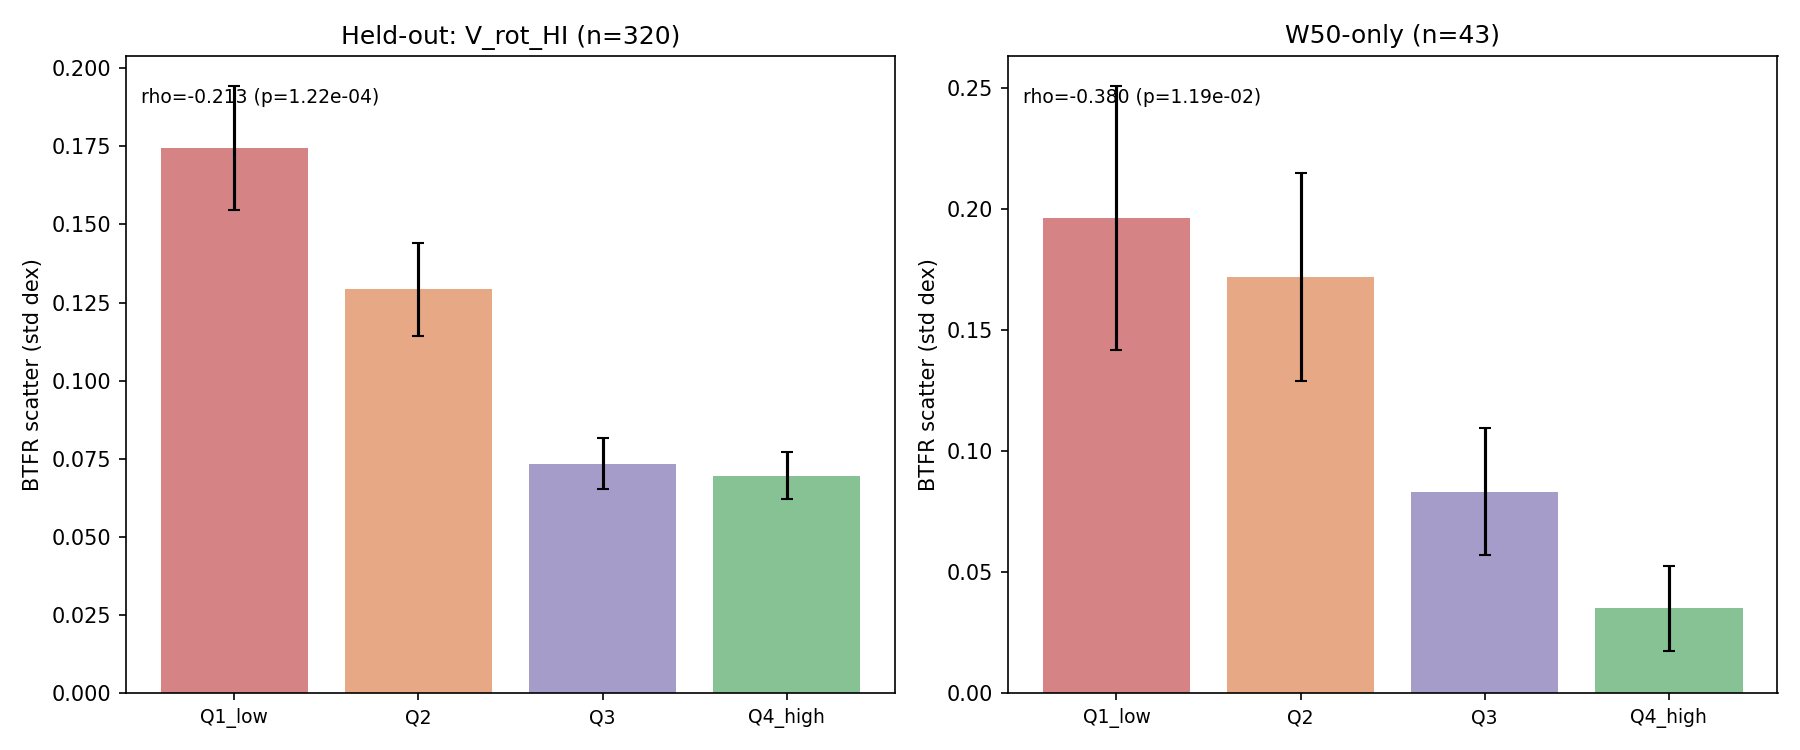
\includegraphics[width=\textwidth]{figures/fig_2_btfr_scatter_by_quartile.png}
\caption{xGASS BTFR residual scatter by organization quartile for two velocity variants. Left: held-out inclination-corrected H~I rotation proxy sample ($N=320$). Right: W50-only subset ($N=43$). Bars show the standard deviation of signed BTFR residuals per quartile; error bars show bootstrap 95\% confidence intervals. The endpoint contrast is present, but intermediate quartiles are not uniformly monotonic.}
\label{fig:scatter_quartile}
\end{figure}

\begin{figure}[H]
\centering
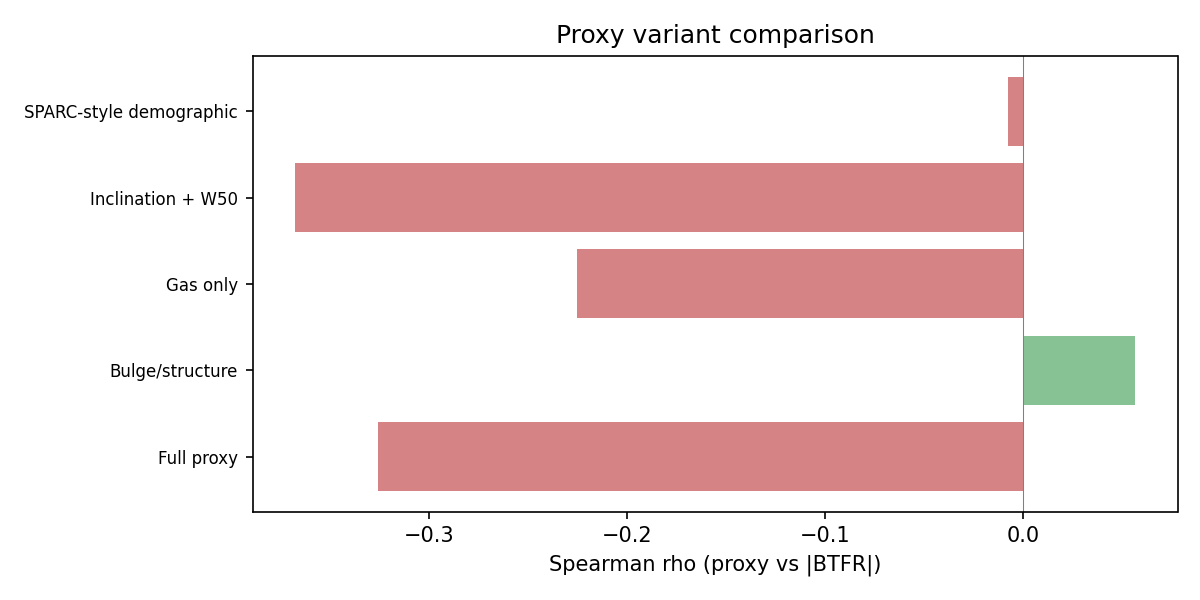
\includegraphics[width=0.75\textwidth]{figures/fig_3_ablation_null_models.png}
\caption{Selected comparison of xGASS proxy variants. Bars show Spearman $\rho$ between each proxy variant and $|\Delta_{\rm BTFR}|$. Kinematics-based proxies (containing inclination and/or linewidth) produce the strongest correlations; gas fraction alone shows the opposite sign.}
\label{fig:ablation}
\end{figure}

\begin{figure}[H]
\centering
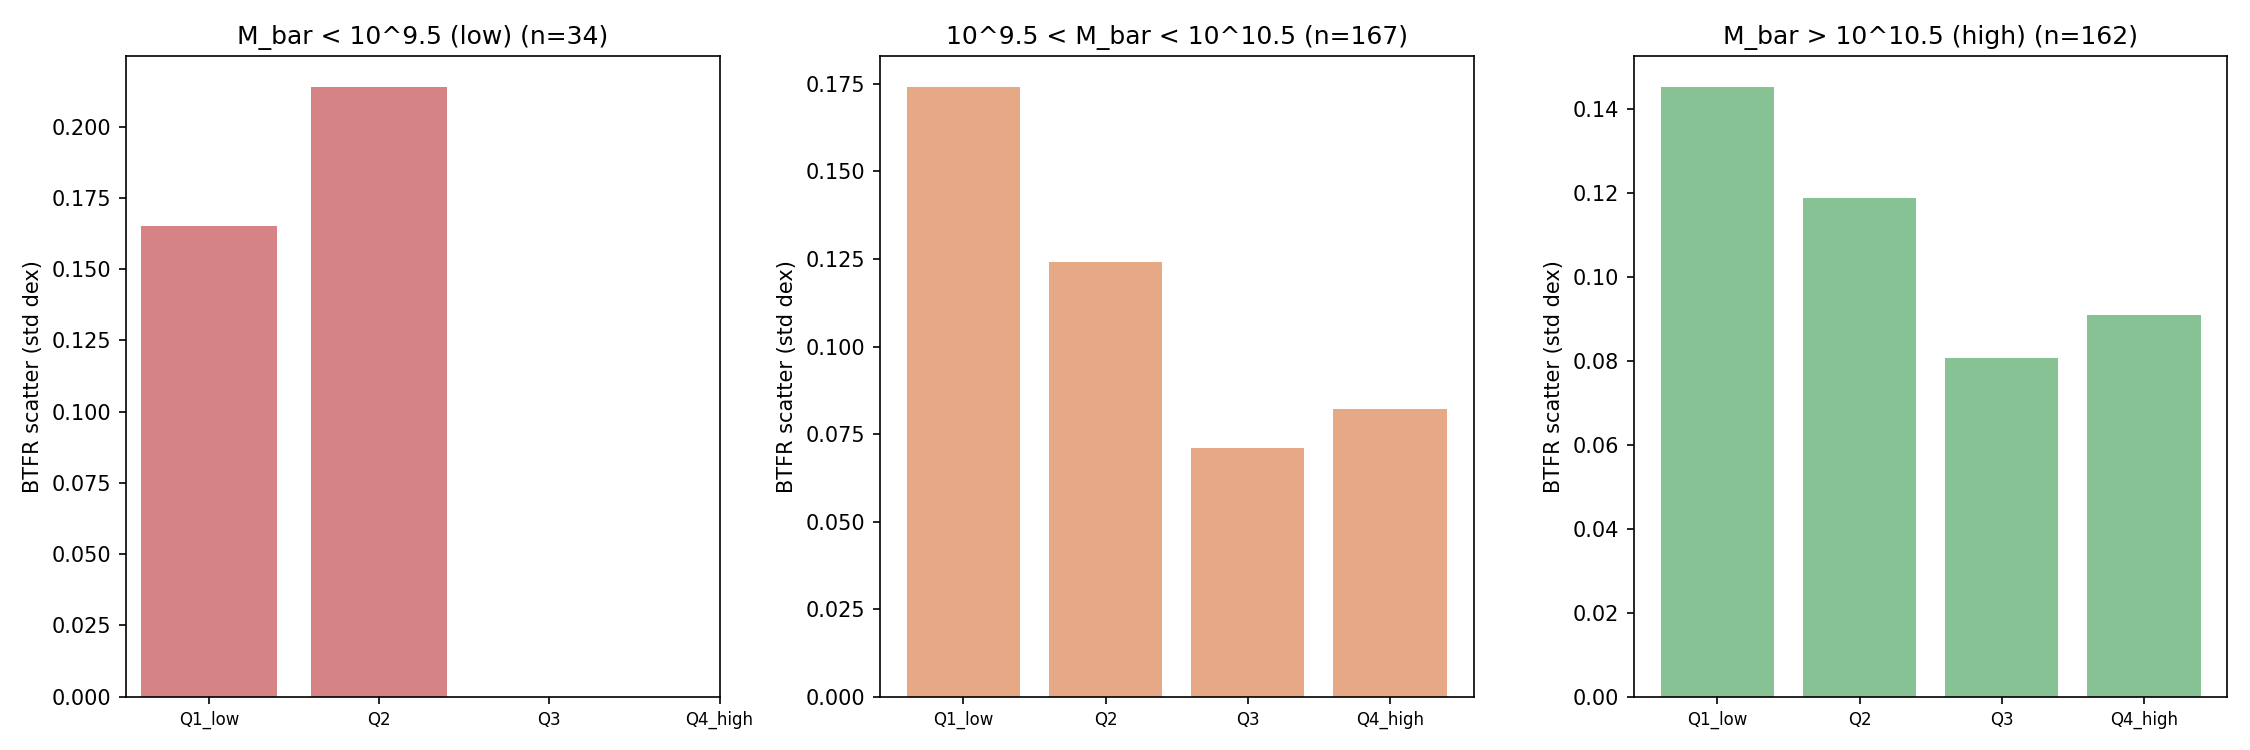
\includegraphics[width=0.75\textwidth]{figures/fig_4_inclination_restricted.png}
\caption{BTFR scatter by organization quartile in three mass bins. The pattern weakens within narrow mass ranges, indicating that mass is a significant confounder. Missing bars indicate quartiles with insufficient objects in that mass bin.}
\label{fig:incl_restricted}
\end{figure}

\begin{figure}[H]
\centering
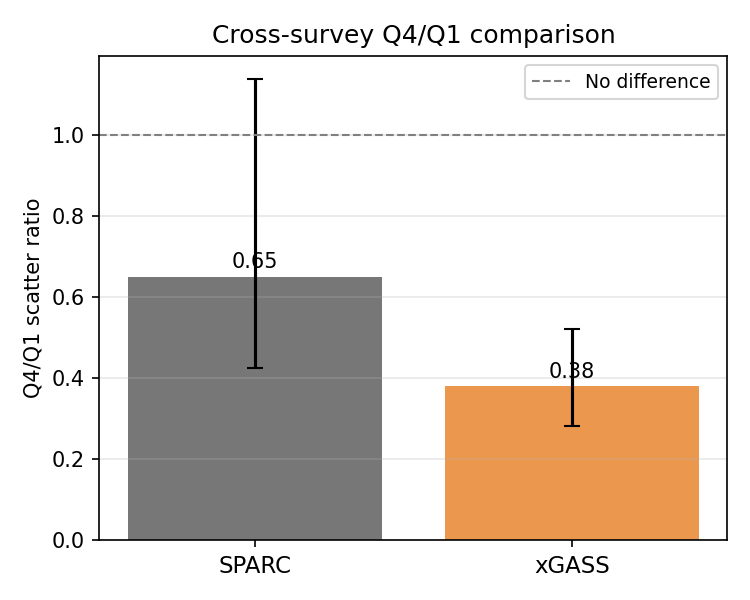
\includegraphics[width=0.75\textwidth]{figures/fig_5_cross_survey_ratios.png}
\caption{Q4/Q1 scatter ratio for SPARC and xGASS. Bars show the within-survey ratio of BTFR residual scatter in the highest-organization quartile to the lowest. Error bars show bootstrap 95\% confidence intervals. The dashed line marks unity (no difference between quartile endpoints). Both point estimates are below unity, indicating directional consistency in the endpoint contrast; the SPARC interval is broad because of the smaller sample.}
\label{fig:cross_survey}
\end{figure}

\begin{thebibliography}{99}

\bibitem[Tully \& Fisher(1977)]{tully1977}
R.~B.~Tully \& J.~R.~Fisher, A\&A, 54, 661 (1977).

\bibitem[Bosma(1978)]{bosma1978}
A.~Bosma, PhD thesis, University of Groningen (1978).

\bibitem[de Blok(2010)]{deblok2010}
W.~J.~G.~de Blok, Adv.~Astron., 2010, 789234 (2010).

\bibitem[McGaugh(2012)]{mcGaugh2012}
S.~S.~McGaugh, AJ, 143, 40 (2012).

\bibitem[Saintonge et al.(2011)]{saintonge2011}
A.~Saintonge et al., MNRAS, 415, 32 (2011).

\bibitem[Lelli et al.(2016)]{lelli2016}
F.~Lelli, S.~S.~McGaugh, \& J.~M.~Schombert, AJ, 152, 157 (2016).

\bibitem[Lelli et al.(2019)]{lelli2019}
F.~Lelli, S.~S.~McGaugh, J.~M.~Schombert, H.~Desmond, \& H.~Katz, MNRAS, 484, 3267 (2019).

\bibitem[Springob et al.(2005)]{springob2005}
C.~M.~Springob, M.~P.~Haynes, \& R.~Giovanelli, ApJS, 160, 149 (2005).

\bibitem[Catinella et al.(2018)]{catinella2018}
B.~Catinella et al., MNRAS, 476, 875 (2018).

\bibitem[Bradford et al.(2016)]{bradford2016}
J.~D.~Bradford, M.~Geha, \& F.~C.~van~den~Bosch, ApJ, 832, 11 (2016).

\bibitem[Verheijen \& Sancisi(2001)]{verheijen2001}
M.~A.~W.~Verheijen \& R.~Sancisi, A\&A, 370, 765 (2001).

\bibitem[Ponomareva et al.(2018)]{ponomareva2018}
A.~A.~Ponomareva, M.~A.~W.~Verheijen, E.~Papastergis, A.~Bosma, \& R.~F.~Peletier, MNRAS, 474, 4366 (2018).

\bibitem[Courteau et al.(2014)]{courteau2014}
S.~Courteau et al., Rev.~Mod.~Phys., 86, 47 (2014).

\bibitem[Oh et al.(2015)]{oh2015}
S.-H.~Oh et al., AJ, 149, 180 (2015).

\bibitem[Schombert et al.(2020)]{schombert2020}
J.~M.~Schombert, S.~S.~McGaugh, \& F.~Lelli, AJ, 160, 71 (2020).

\bibitem[Navarro et al.(1997)]{navarro1997}
J.~F.~Navarro, C.~S.~Frenk, \& S.~D.~M.~White, ApJ, 490, 493 (1997).

\bibitem[Mo et al.(1998)]{mo1998}
H.~J.~Mo, S.~Mao, \& S.~D.~M.~White, MNRAS, 295, 319 (1998).

\bibitem[McGaugh(2004)]{mcGaugh2004}
S.~S.~McGaugh, ApJ, 609, 652 (2004).

\bibitem[Swaters et al.(2009)]{swaters2009}
R.~A.~Swaters, R.~Sancisi, T.~S.~van~Albada, \& J.~M.~van~der~Hulst, AJ, 138, 1113 (2009).

\bibitem[Famaey \& McGaugh(2012)]{famaey2012}
B.~Famaey \& S.~S.~McGaugh, Living Rev.~Rel., 15, 10 (2012).

\bibitem[Pillepich et al.(2019)]{pillepich2019}
A.~Pillepich et al., MNRAS, 490, 3196 (2019).

\bibitem[Walter et al.(2008)]{walter2008}
F.~Walter et al., AJ, 136, 2563 (2008).

\bibitem[Wisnioski et al.(2015)]{wisnioski2015}
E.~Wisnioski et al., ApJ, 799, 209 (2015).

\end{thebibliography}

\end{document}
